\section{Introduction}
\label{sec:intro}

Personalized recommendation is a critcal component for most web
systems, including online advertising, e-commerce websites, social
network, etc. Let's take online advertising as an example. It's a
multi-billion dollar business, accounts for majority of the revenue
for companies like Google and Facebook. It's also the main income
source for millions web content publishers and most e-commerce
websites. Therefore, the impact of designing good personalized
recommendations is huge.

In this paper, we present an innovative machine learning model for
personalized recommendations that can handle extremely sparse and
large scale data. Since our team works on the personalized keyword
recommendation for advertisers in Google Adsense~\cite{adsense:wiki},
for the rest of this paper, we will use our project as an example. But
by no means our model is limited to this example. It can be easily
applied to other personalized recommendation systems.

Google Adsense allows publishers in the network of content sites to
serve automatic advertisements (for text, image, videos, or
interactive media), which are targeted to site content and
audience. It generates billions of dollars each year, supports
hundreds of millions of publishers on the Internet eco-system, and can
reach more than 80\% of all Internet users worldwide in more than 30
languages and over 100 countries. All these make it one of advertiser'
favorite online advertising systems. In a nutshell, how it works can
be illustrated by Figure~\ref{fig:adsense}.
\begin{itemize} \itemsep -1pt
\item {\em Publisher} posts content on the Internet, and insert a code
  snippet into its web pages.
\item {\em User} visits the web page, which triggers the code snippet
  to pull relevant advertisements from Google Adsense servers, and
  show them on the same web page.
\item If user click on the advertisement, the {\em advertiser} who
  created it will pay Google certain amount of money, and Google will
  share majority of that payment with the content publisher.
\end{itemize}

\begin{figure}[!ht]
  \centering
  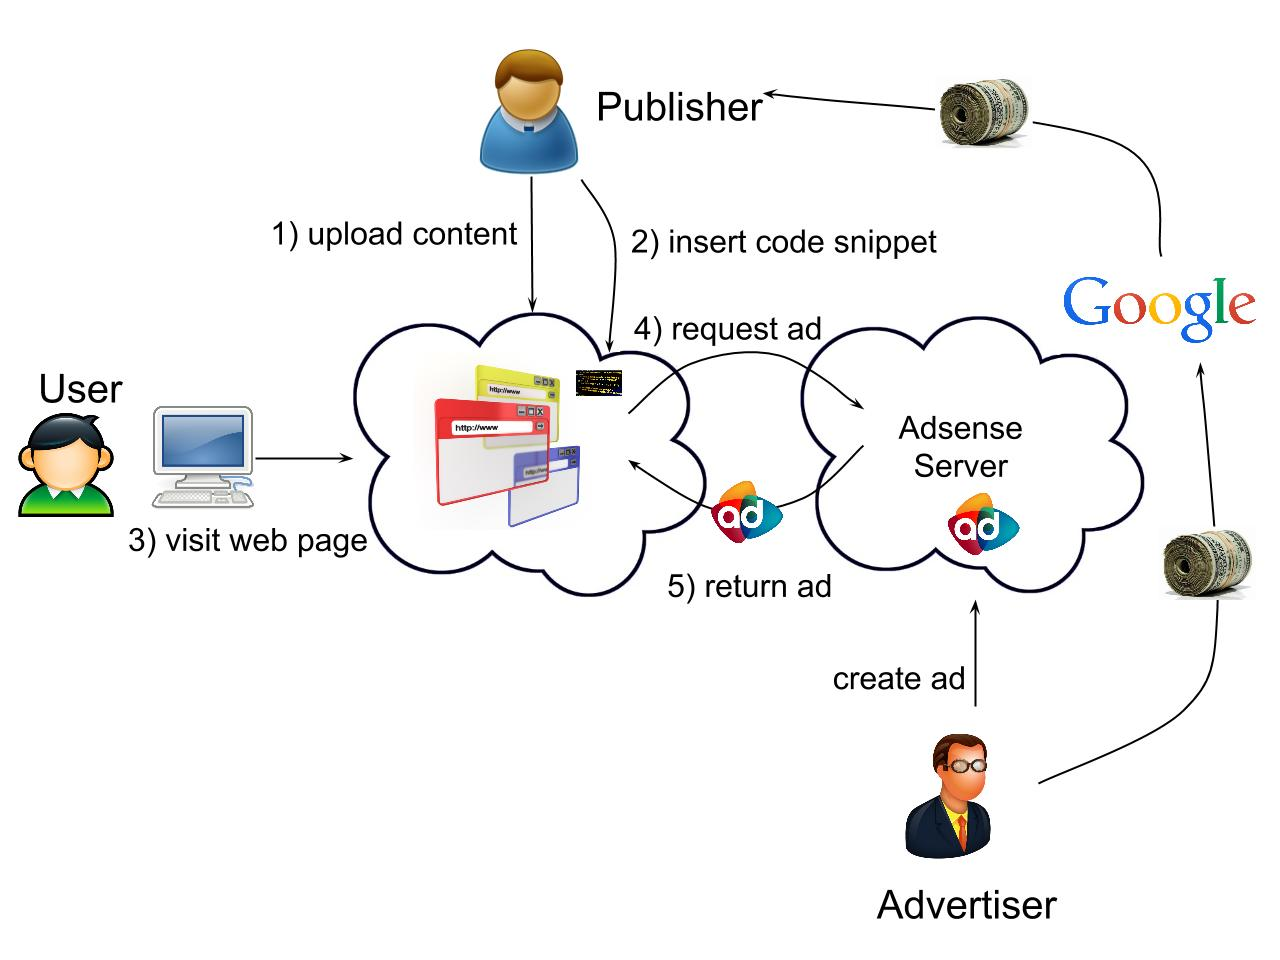
\includegraphics[width=0.4\textwidth]{figures/adsense.jpg}
  \caption{Google Adsense system work flow.}
  \label{fig:adsense}
\end{figure}

To make the best out of Adsense, it requires the advertisers to
provide a good list of keywords, to match advertisements with web
contents more precisely, hence increase the click through rate and
better advertisement performance. However, the reality is most
advertisers are lack of experience to provide good keywords for their
advertisements. Therefore, intelligently making use of historical data
to provide good personalized keyword recommendations to advertisers is
crutial to the success of Adsense. There are mainly two types of
approaches.
\begin{itemize}
\item A/B-testing~\cite{abtest:wiki}. In this approach, we split the
  web traffice into two parts: majority of the traffic uses the
  original keyword list to match advertisement, and the other small
  fraction of the trafic uses the new keyword list (original keyword
  list along with some semantically relevant keywords). Do this
  experiment for some period of time (usually in days or weeks) and
  compare the stats. If the new list performs significantly better, we
  then surface this recommendation to the advertiser. The main
  drawback of this approach is the long turnaround time. Lots of
  business opportunities may be lost after days or weeks of
  experiments.
\item Model based solutions using collaborative
  filtering~\cite{resnick1997recommender,sarwar2001item}. This
  approach makes use of machine learning technology and predicts the
  performance of the new keyword list without running
  experiments. There are three type of collaborative filtering models
  that are commonly used, user neighborhood model (considering the
  similarity between users, in our case will be advertisers), item
  neighborhood model (considering the similarity between items, in
  oursecase will be keywords), and matrix factorization based
  model~\cite{}. The matrix factorization based model has drawn a lot
  of attention recently due to its success in the Netflix
  Challenge~\cite{}. It's proven to produce better estimates than user
  neighborhood or item neighborhood models, and can handle sparse data
  set like the data in Netflix Challenge. However, the data set we
  deal with is more than 100 times sparser than the Netflix data. We
  observe significant overfitting even with very strong
  regularization.
\end{itemize}

As a result, we went out and designed a novel new machine learning
model that is resilient to extremely sparse data set and doesn't need
to run days of experiments. First, the complexity of the model
(a.k.a. the number of parameters) grows with respect to observed data,
not to the number of advertisers and number of keywords like matrix
factorization based models. This makes our model resilient to
extremely sparse data. Secondly, our training algorithm is based on
gradient descent, which is easy to parallelize, and thus can handle
very large scale data set. Thirdly, our model combines the user
neighborhood and item neighborhood ideas in collaborative filtering
smartly, where similarities are ``learned'' from training algorithm
other than defining a global similarity metric for neighborhood. This
makes the estimation quality of our model very good.

In summary, our main contributions in this paper include:
\begin{itemize} \itemsep -1pt
\item We successfully exploit the potential of improving personalized
  recommendation for extremely sparse and large scale data.
\item Novel ideas in model design include: (a) control model
  complexity with respect to observed data; (b) intelligently combine
  ideas in collaborative filtering.
\item We have applied our model successfully to personalized keyword
  recoomendation system in Google Adsense. And we have conducted
  extensive comparison experiments with matrix factorization based
  methods.
\item We have implimented a distrubted training system that can handle
  large scale data set and is ready to apply to other personalized
  recommendation problems.
\end{itemize}

The remainder of this paper is organized as follows. We first
formulate the problem in Section~\ref{sec:problem}. Then we describe
the details of our model, including the high-level workflow, intuition
and assumptions, as well as different components of the model in
Section~\ref{sec:model}. After that, we introduce the training
algorithms in Section~\ref{sec:trainer}. We present experimental
results in Section~\ref{sec:exp}, and related works in
Section~\ref{sec:related}. Finally, we conclude this paper in
Section~\ref{sec:conclusion}.
